\chapter*{}
%\thispagestyle{empty}
%\cleardoublepage

%\thispagestyle{empty}

\begin{titlepage}
 
 
\setlength{\centeroffset}{-0.5\oddsidemargin}
\addtolength{\centeroffset}{0.5\evensidemargin}
\thispagestyle{empty}

\noindent\hspace*{\centeroffset}\begin{minipage}{\textwidth}

\centering
%
\includegraphics[width=0.9\textwidth]{imagenes/logo_ugr.jpg}\\[1.4cm]

%\textsc{ \Large PROYECTO FIN DE CARRERA\\[0.2cm]}
%\textsc{ INGENIERÍA EN INFORMÁTICA}\\[1cm]
% Upper part of the page
% 

 \vspace{2.3cm}

%si el proyecto tiene logo poner aquí
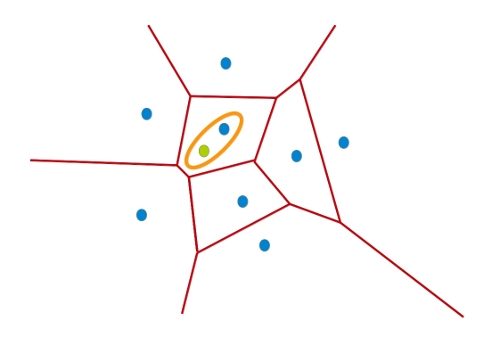
\includegraphics[scale=0.5]{imagenes/logo_voronoi.jpg} 
 \vspace{0.5cm}

% Title

{\Huge\bfseries Diagramas de Voronoi\\
}
\noindent\rule[-1ex]{\textwidth}{3pt}\\[3.5ex]
{\large\bfseries Librería para el cálculo y gestión de Diagramas de Voronoi.\\[4cm]}
\end{minipage}

\vspace{2.5cm}
\noindent\hspace*{\centeroffset}\begin{minipage}{\textwidth}
\centering

\textbf{Autora}\\ {María Oliver Balsalobre (alumno)}\\[2.5ex]
\textbf{Director}\\
{Daniel Sánchez Fernández (tutor)}\\[2cm]

\end{minipage}
\vspace{\stretch{2}}

 
\end{titlepage}





\cleardoublepage

\chapter*{}

\pagestyle{empty}

\begin{center}
{\large\bfseries Librería para el cálculo y gestión de Diagramas de Voronoi}\\
\end{center}
\begin{center}
María Oliver Balsalobre (alumna)
\end{center}

\vspace{0.7cm}
\noindent{\textbf{Palabras clave}: Diagrama de Voronoi, Triangulación de Delaunay, Algoritmo, Puntos, Vértices }\\

\vspace{0.7cm}


\centerline{\textbf{Resumen}}
\addcontentsline{toc}{chapter}{Resumen}

\bigskip

En este Trabajo Fin de Grado se aborda el problema de los Diagramas de Voronoi y su dual, es decir, la triangulación de Delaunay. Dado que nuestros objetivos principales eran elaborar una librería para el cálculo y gestión de estos diagramas en espacios euclídeos y su previo estudio en diversas tipologías, propiedades y algoritmos de obtención, comenzamos el trabajo con una serie de resultados previos sobre los que hablaremos durante el transcurso del proyecto.

Tras definir estos conceptos de vital importancia, en el tercer capítulo daremos una normalización del Diagrama de Voronoi, una de las estructuras fundamentales dentro de la Geometría Computacional, que se define como la descomposición de un espacio métrico en regiones de forma que a cada objeto se le asigna una región del espacio métrico formada por los puntos que están más cerca de él que de ningún otro objeto. Comentaremos algunas de sus propiedades y las numerosas aplicaciones que utilizan estos diagramas además de situaciones de nuestro día a día en las que podemos encontrarnos esta estructura. Además, en la elaboración práctica y el desarrollo informático de este trabajo llevaremos a cabo una de estas aplicaciones: robótica; los robots intentan llegar a un lugar indicado evitando obstáculos.

También hablaremos de la Triangulación de Delaunay, el dual del Diagrama de Voronoi, ya que los circuncentros que quedan tras hacer esta triangulación, son los vértices de las aristas que forman dicho Diagrama de Voronoi. Mencionaremos también algunas de sus propiedades básicas ya que esta triangulación posee varias características acerca de sus propiedades de optimización, sus estructuras como subgrafo y su flexibilidad para adaptarse a todo tipo de dimensiones. Comentaremos el algoritmo del vecino más cercano, un problema de distancia que se resuelve directamente con el Diagrama de Voronoi y veremos que podemos calcular un par de puntos cuya distancia es mínima si el vecino más cercano para cada punto dentro de nuestro conjunto es conocido.

A continuación analizaremos algunos de los algoritmos estudiados para el cálculo tanto de los Diagramas de Voronoi como para la triangulación de Delaunay y veremos que este capítulo se encuentra a caballo entre los dos temas principales de nuestro trabajo: la geometría y la computación. Estos algoritmos nos serán muy útiles en el desarrollo y realización de la librería, para su cálculo y gestión y tendremos en cuenta en todo este apartado el concepto de orden de complejidad definido en el capítulo 3, para entender a qué nos referimos al hablar de tiempo empleado en los distintos algoritmos. 

En la siguiente sección haremos, en primer lugar, un análisis de los requisitos donde describiremos detalladamente el comportamiento de nuestro sistema, los datos que recibe, trata, almacena y devuelve y cualquier consideración sobre su funcionamiento. Detallaremos cómo hemos resuelto el problema planteado, elaborando una librería mediante el lenguaje de programación Java cuya utilización por un lado, nos va a permitir, al pasarle un fichero de texto con la entrada correspondiente, obtener la salida deseada que será la dimensión, el número de puntos y las coordenadas de dichos puntos, que serán los vértices de Voronoi y por último, el número de regiones (polígonos) de Voronoi. Por otro lado, en otro proyecto realizaremos el diseño gráfico del Diagrama de Voronoi, incluyendo la librería realizada con una serie de clases que serán la base de la implementación. Para finalizar este capítulo elaboraremos un manual de usuario en el que se explicará paso a paso y de forma detallada y amigable para cualquier usuario, el funcionamiento de las dos aplicaciones desarrolladas. 

Por último, en la finalización de este trabajo, haremos una autoevaluación en la que veremos si se han cumplido los objetivos planteados al inicio del proyecto y comentaremos la aportación personal que ha supuesto su realización, así como la mención de algunas vías futuras interesantes que son consecuencia de la investigación realizada.







\cleardoublepage

\chapter*{}

\thispagestyle{empty}


\begin{center}
	{\large\bfseries Voronoi Diagrams: Library for the calculation and management of Voronoi Diagrams.}\\
\end{center}
\begin{center}
	María Oliver Balsalobre (student)\\
\end{center}

\vspace{0.7cm}
\noindent{\textbf{Keywords}: Voronoi Diagrams, Delaunay Triangulation, Algorithm, Points, Vertex}\\

\vspace{0.7cm}
\centerline{\textbf{Abstract}}
\addcontentsline{toc}{chapter}{Abstract}

\bigskip 

This project verses about the known problem of Voronoi Diagrams along with its dual counterpart, Delaunay triangulation. One of the main objectives has been to create a library for the calculation and handling of these diagrams in Euclidean spaces, including preliminary analysis on different typologies, properties and building algorithms. A series of previous results has been used as a starting point to develop the whole topic discussion along this project.

As a starting point, key concepts are described and detailed, providing a normalization for the Voronoi Diagram which is one of the fundamental structures in Computational Geometry. Its origins in the Western literature date back to at least 17th century. René Descartes claims that the solar system consists of vortices.  His illustrations show a descomposition of space into convex regions, each consisting of mater revolving around one of the fixed stars. Even thoug Descartes has not explicitly defined the extension of these regions, he gave us the underlying idea. Formally, Voronoi Diagrams are defined as the decomposition of a metric space in regions, in a way that every object is allocated a region of the metric space, composed by the closest points to that specific object. A Voronoi region is then defined as the group of closest points to any given point, and a Voronoi edge will be the boundary between two Voronoi regions. One of the main properties discussed implies that a convex partition of the plane defines a Voronoi diagram if and only if there is only one unique point for each region. 

Indeed, this fundamental concept has emerged independently, and proven useful, in various fields of science. It is important to highlight how present Voronoi Diagrams are in many different fields and disciplines such as architecture, design, urban building or meteorology. Indeed the practical side of this project uses one specific example of Voronoi Diagrams application: robotics, where robots follow certain pre-established path, avoiding obstacles along the way.

When talking about Delaunay Triangulation, the link with its dual counterpart, Voronoi Diagram, is drew, as building one of them immediately enables the construction of the other: the circumcentres obtained by the triangulation would be the vertexes for the edges of the Voronoi Diagram. Formally, a network of triangles becomes a Delaunay Triangulation if all the circumscribed circumferences being part of the triangles of the network are empty, meaning that no other vertexes are included, apart from the three vertexes defining them. As part of the dissertation, some basic properties of this triangulation will be presented, related to optimization capabilities, subgraph structures and flexibility to adapt itself to any number of dimensions. The nearest neighbour algorithm will be tackled, a known distance problem that can be directly resolved using the Voronoi diagrams. One important aspect is how to calculate a pair of points separated by the minimum distance, giving that the nearest neighbour for each point of the group is known. And this will be done in a lineal space and time.



Geometry and its link to computation complexity is an important part of this exercise, focusing on the variety of algorithms that can be used to calculate both the Voronoi Diagrams and Delaunay Triangulations. The brute force algorithm is explained, as a first approach, being a way to explore the geometry of each Voronoi region. Then the incremental algorithm is discussed, generally based in building the k points diagram and then move to the k+1 points version. Additionally, Bowyer-Watson algorithm is described, detailing how it can be used to calculate the Delaunay triangulation of a finite set of points for any number of dimensions. One further step will deal with the divide and conquer algorithm, explaining its associated high complexity while being the optimum method for the deterministic worst case. And finally the Fortune algorithm, based on a plain sweep technique, which on one hand can calculate the Voronoi Diagram for a cloud of points in the plane, but on the other hand it is by far the most complex approach. These algorithms will be a key part of the library being built, and the complexity measurement will be a very important input for its design (including the constant / logarithmic / lineal order), when talking about time taken by each of the algorithms to solve the given problem. A full set of functions will be created, sharing the same asymptotic behaviour that will lead to understanding which algorithms are the most efficient ones among the selection. 

Once the algorithm screening is finished, the focus goes to the system that has been built, analysing the initial requirements and the expected behaviour, including inputs expected, how they are handled and stored, and outcomes. The solution to the initially defined problem is detailed, using the library programmed in Java, that potentially could be used by anyone to resolve this specific problem or adapting it for other use cases. Some defined classes are key to understand how the library has been built: “Punto”, where the points defining the Euclidean space are grouped, as well as basic geometric calculations and the representation of matrixes and convex hulls; “Conjunto”, which is an abstract class built to create the skeleton of the interface, essentially being the body of the implementation; “Triangulo”, which inherits from the previous class, enabling the calculation of the neighbour triangles, the circumcentres and the opposite side to an any given vertex; “Grafo”, which will sustain the graph development, adding or subtracting both nodes and edges in the undirected graph, and will provide the set of nodes for the specific graph; “Triangulacion2D” will calculate the 2D Delaunay triangulation itself using the incremental algorithm, as, though not being the optimum or fastest approach, facilitates an interactive way of understanding and seeing how the algorithm works; and finally “Dijkstra”, specific class implementing the Dijkstra algorithm, calculating the shortest way from one point of the graph to any other point, taking into account the weight of each edge.

The system will work as follows: as an input we will use a text file that will contain the expected dimension, the number of points and their coordinates; and the outcome will be the Voronoi vertexes coordinates and the number of Voronoi regions (polygons). Additionally, the graphic representation of the Voronoi diagram in 2D has been implemented, including a library built over JFrame and using JPanel (Java tools). Within the JPanel, all the different methods available to build the Voronoi Diagrams and its associated Delaunay Triangulations have been implemented, along with the circumscribed circumferences. Different basic and specific drawing approaches are available, apart from a list of methods to calculate the shortest path between two random points. Using JFrame, the whole interactive framework is provided, enabling the user to work with the tool in real time.

As a complement, a user manual has been written, including a step by step guideline for both developed applications, that is, the graphic representation of the Voronoi Diagram and tools to support the input and output of terminal data. Screenshots for each part have been included as a way to facility the usage of the different options available. It is important to highlight that there are two different modes of operation: Voronoi, being the default option, to calculate the Voronoi Diagram for the set of points provided as an input; and Dijkstra, that will provide the option of choosing two random points, calculating the shortest path between them through the Voronoi vertexes and edges. Additionally, extra information can be displayed to describe the Delaunay Triangulation or the circumscribed circumferences to each triangle, associated to the created Voronoi Diagram. Basic interaction with the files has been included for simplicity, so open, save and export functions have been added to the interface. Furthermore, other options have been developed to facilitate user interaction such as erasing the whole palette to start from scratch, seeing or hiding the tool bar, zooming in the diagram, or provide new points by entering its coordinates instead of using the click button. As already mentioned, both applications are available for anyone to use them or build up on them to expand the use cases or problems that could provide a solution for.

As a set of next steps, based on the outcome of this study, different options to continue the investigation are described. The body of literature on Voronoi Diagrams is vast and continuously growing, and many of the arising both theoretical and practical problems have found elegant and efficient solutions. Naturally, new questions have emerged from the exhaustive research conducted, and quite a few problems eluded satisfactory settlement until today. Especially those problems related to both the combinatorial complexity of simple structures and their efficient algorithm construction are still to be further investigated and resolved when dealing with Voronoi Diagrams. Therefore, as an interesting example, future work could be focused on Voronoi Diagrams of circles, and its application to the visualization of the growth of particles, studying Peter Gärdenfors’ theory of conceptual representations, as a bridge between the symbolic and connectionist approaches, just to mention one of the multiple interesting ways forward.



\chapter*{}
\thispagestyle{empty}

\noindent\rule[-1ex]{\textwidth}{2pt}\\[4.5ex]

Yo, \textbf{María Oliver Balsalobre}, alumna de la titulación Doble Grado en Ingeniería Informática y Matemáticas de la \textbf{Facultad de Ciencias} y la \textbf{Escuela Técnica Superior de Ingenierías Informática y de Telecomunicación de la Universidad de Granada}, con DNI 75719191-V, autorizo la ubicación de la siguiente copia de mi Trabajo Fin de Grado en la biblioteca del centro para que pueda ser consultada por las personas que lo deseen.
\begin{figure}  [H]
    \centering
    
\includegraphics[scale=0.5]{imagenes/firmaMaria.JPG}
\end{figure}
\vspace{3cm}

\noindent Fdo: María Oliver Balsalobre

\vspace{2cm}

\begin{flushright}
Granada a 26 de Junio de 2017 .
\end{flushright}


\chapter*{}
\thispagestyle{empty}

\noindent\rule[-1ex]{\textwidth}{2pt}\\[4.5ex]

\textbf{Daniel Sánchez Fernández}, Profesor del Área de Bases de Datos Inteligentes y Sistemas de Información de la Universidad de Granada.

\vspace{0.5cm}

\textbf{Informa:}

\vspace{0.5cm}

Que el presente trabajo, titulado \textit{\textbf{Librería para el cálculo y gestión de Diagramas de Voronoi}}, ha sido realizado bajo su supervisión por \textbf{María Oliver Balsalobre (alumna)}, y autorizo la defensa de dicho trabajo ante el tribunal que corresponda.

\vspace{0.5cm}

Y para que conste, expiden y firman el presente informe en Granada a 26 de Junio de 2017.

\vspace{1cm}

\textbf{El tutor:}

\begin{figure}  [H]
    \centering
    
\includegraphics[scale=0.7]{imagenes/firmaDani.JPG}
\end{figure}

\vspace{3cm}

\noindent \textbf{Daniel Sánchez Fernández}

\chapter*{Agradecimientos}
\thispagestyle{empty}

Gracias a mi tutor Daniel, por ayudarme en todo lo posible desde el primer momento y haber estado disponible cada vez que lo he necesitado para contribuir con sus conocimientos a la realización de este trabajo.
\vspace{0.5cm}

Gracias a mi familia, en especial a mis padres, mis hermanos y mis abuelos, por el apoyo incondicional y constante. Gracias por haberme enseñado, tanto en lo personal como en lo profesional, y por el amor que recibo a diario.
\vspace{0.3cm}

Gracias a mis compañeros por recorrer juntos este camino hacia el final del Doble Grado y por pasar conmigo momentos inolvidables.
Solís, eres la persona con las mejores ideas para resolver problemas que he conocido durante estos años y fundamental para mí.
Marc estoy orgullosa de ti por todo lo que has conseguido y sigues consiguiendo. Me encanta verte crecer en lo que te gusta.
Torres sabes que soy tu fan número uno, eres una de las mejores personas que conozco.
Ramón, espero que de todos estos años te lleves un buen recuerdo de lo que hemos compartido durante la carrera tal y como lo haré yo.
Miki, me alegro mucho de haberte conocido y haber compartido tantos momentos juntos, tanto profesionales como personales durante la carrera.
\vspace{0.5cm}

Gracias a mis amigos, los de siempre (CarmenAG, Mmar, Tina, Eli, Ajo, Paquito, Dani), por aguantar mis cambios de humor, estar siempre dispuestos a escucharme y ser un pilar imprescindible en mi vida.
Dicen que los amigos son la familia que se elige y sin duda, yo no podría haber elegido mejor.
\vspace{0.5cm}

Y a mi mejor amigo, compañero de vida y de experiencias, y mi primer y último pensamiento en todo lo que hago, gracias por todo, espero pasar toda una vida juntos y seguir viéndote crecer y consiguiendo todas tus metas y objetivos.
\vspace{0.5cm}

Sin vosotros terminar el Doble Grado en Ingeniería Informática y Matemáticas no habría sido posible.